\section{Background}

\begin{frame}
        \centering
        \huge Background
\end{frame}

\begin{frame}
	\frametitle{Field}
	\begin{columns}
		\begin{column}{0.4\textwidth}
			\begin{itemize}
				\item Social Networks
				\item Network Diffusion
				\item Source Detection
			\end{itemize}
		\end{column}
		\begin{column}{0.6\textwidth}
			\begin{figure}
				\centering
				
\includegraphics[scale=0.2]{fb-art.png}
				\caption{Facebook}
			\end{figure}
			\begin{figure}
				\centering
				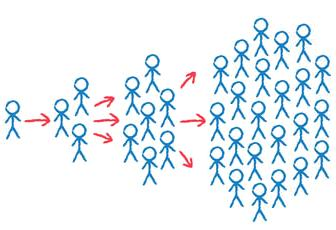
\includegraphics[scale=0.3]{socialnetwork.jpg}
			\end{figure}
			\footnotetext{ https://www.linkedin.com/pulse/20140918141439-7859692-social-network-301-what-is-virality}
		\end{column}
	\end{columns}
	\note{The field of source detection}
\end{frame}

\begin{frame}
	\frametitle{Contributions}
	\begin{itemize}
		\item Introducing representation learning approach to the field of source detection delivering a robost model that handles data sparsity well
		\item Does not require the influence graph to be known
		\item Tested on real life data and surpassing other baseline approaches
		\item Provides an extension that further improves the results
	\end{itemize}
	\note{
		\begin{itemize}
			\item a
		\end{itemize}
		}
\end{frame}